\usetikzlibrary{positioning,arrows,calc}

\tikzset{
modal/.style={>=stealth’,shorten >=1pt,shorten <=1pt,auto,node distance=1.5cm,
semithick},
world/.style={circle,draw,minimum size=0.5cm,fill=gray!15},
point/.style={circle,draw,inner sep=0.5mm,fill=black},
reflexive above/.style={->,loop,looseness=7,in=120,out=60},
reflexive below/.style={->,loop,looseness=7,in=240,out=300},
reflexive left/.style={->,loop,looseness=7,in=150,out=210},
reflexive right/.style={->,loop,looseness=7,in=30,out=330}
}

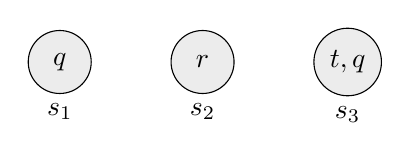
\begin{tikzpicture}[world/.append style={minimum size=0.8cm}, x=1cm,y=1cm]

\node[world] (s1) [label=below:$s_1$] {$q$};
\node[world] (s2) [label=below:$s_2$,right=of s1] {$r$};
\node[world] (s3) [label=below:$s_3$,right=of s2] {$t,q$};

\end{tikzpicture}